\section{Exercises from Lecture 6}

%%%%%%%%%%%%%%%%%%%%%%%%%%%%%%%%%%%%%%%%%%%%%%%%%%%%%%%%%%%%%%%%%%%%
\subsection{Exercise 6.15}
\emph{Consider the double integrator}
\begin{align}
    &\Dot{x}_1(t) = x_2(t), \\
    &\Dot{x}_2(t) = u(t)
\end{align}
\emph{and the cost}
\begin{equation}
    J(u) = \int_{t_0}^\infty \left( x_1(t)^2 + x_2(t)^2 + u(t) ^2 \right) dt
\end{equation}
\emph{Find P by solving the ARE. Verify (either analytically or numerically) that it is indeed the steady-state solution of the RDE.}
\\
\\
\textbf{Solution:}\\
\\
In order to solve the Algebraic Riccati Equation, we have to find the matrices defining the system. In this case, we have:
\begin{equation}
    A = \begin{bmatrix}
         0 & 1 \\
         0 & 0 \\
    \end{bmatrix}
    ,\smallspace B=
    \begin{bmatrix}
         0 \\
         1 \\
    \end{bmatrix}
    , \smallspace Q =
    \begin{bmatrix}
         1 & 0\\
         0 & 1\\
    \end{bmatrix}
    , \smallspace R =
    \begin{bmatrix}
         1 \\
    \end{bmatrix}
\end{equation}
We can now use the Python's library \href{https://www.scipy.org/}{SciPy} to solve the ARE:

\begin{minted}{python}
# Importing the packages
import numpy as np
from scipy.linalg import solve_continuous_are

# Build matrices
A = np.matrix([[0, 1],
               [0, 0]])
B = np.matrix([[0],[1]])
Q = np.eye(2) # Identity matrix, dim = 2
R = np.eye(1) # Identity matrix, dim = 1

# Solve the ARE
P = solve_continuous_are(A, B, Q, R)
print(P)
\end{minted}

By which we get 
\begin{equation}
    P = \begin{bmatrix}
         1.73205081 & 1 \\
         1 & 1.73205081 \\
    \end{bmatrix}
    \sim \begin{bmatrix}
         \sqrt{3} & 1 \\
         1 & \sqrt{3} \\
    \end{bmatrix}
\end{equation}

The formula for Riccati Differential Equation is as following:
\begin{equation}
    \Dot{P}(t) = -P(t)A - A^\top P(t) -Q + P(t) B R^{-1} B P(t) 
\end{equation}
So, based on the previous result we can get $ \Dot{P}(t) $ as following
\begin{minted}{python}
# Calculate the steady-state derivative
P_dot = A.T*P + P*A + Q -P*B*R*B.T*P 
print(P_dot)
\end{minted}
By which we get 
\begin{equation}
    \Dot{P} = \begin{bmatrix}
         0 & 0\\
         0 & 0\\
    \end{bmatrix}
\end{equation}
hence proving P is indeed the steady-state solution of the RDE.


%%%%%%%%%%%%%%%%%%%%%%%%%%%%%%%%%%%%%%%%%%%%%%%%%%%%%%%%%%%%%%%%%%%%
\subsection{Exercise 6.24}
\emph{Consider the infinite-horizon LQR problem}
\begin{align}
    &u^* := \argmin_{u:[0,\infty) \to \mathbb{R}} J(u) := \int_0^\infty \left( qx(t)^2 + ru(t)^2  \right) dt \\
    &\text{subject to}\\
    &\Dot{x}(t) = ax(t) + bu(t), \smallspace t \in [t_0, \infty) \\
    &x(t_0) = x_0
\end{align}

\emph{where $a, q, r > 0$ and $b \in \mathbb{R}$ is arbitrary. Find the optimal control law. Moreover, show that for $r \to 0 $,
the eigenvalue of the optimal closed-loop system moves off to $- \infty$, while for $r \to \infty$, the eigenvalue of the
optimal closed-loop system tends to $−a$}
\\
\\
\textbf{Solution:}\\
\\
Recalling the ARE as:
\begin{equation}
    0 = A^\top P + PA + Q -PBR^{-1}B^\top P
\end{equation}
the optimal control law will be given by:
\begin{align}
    &u^*(t) = K x^*(t)\\
    &\text{where the gain } K = -R ^{-1} B^\top P
\end{align}
with $P$ being the solution to the ARE. In this case, we have scalars instead of matrices, so the ARE becomes
\begin{align}
    &0 = aP + Pa +q - pb\frac{1}{r}bp\\
    &\Longrightarrow -\frac{b^2 P^2}{r} + 2aP + q = 0
\end{align}
Solving the equation, we get as a solution (choosing the positive sign, since we have the condition that $P \geq 0$):
\begin{equation}
    P = \frac{r \left(a  + \sqrt{a^2 + \frac{b^2 q}{r}} \right)}{b^2} 
\end{equation}

Therefore, the closed-loop gain $K$ becomes:
\begin{equation}
    K = - \frac{1}{r} b \frac{r \left(a +  \sqrt{a^2 + \frac{b^2 q}{r}} \right)}{b^{2}} = - \frac{a + \sqrt{a^2 + \frac{b^2 q}{r}}}{b}
\end{equation}
where $K \in \mathbb{R}$. The closed-loop system becomes:
\begin{equation}
    \Dot{x}^*(t) = Ax^*(t) + Bu^*(t) = (a - Kb)x^*(t)
\end{equation}
The eigenvalue of the closed loop system is the value of the scalar $a - Kb$ in this case.
\paragraph{Eigenvalues of the closed-loop system by changing $r$}
\begin{itemize}
    \item Case 1: $r \to 0$, we have the following limit for the gain $K$
    \begin{equation}
        \lim_{r \to 0} (a - Kb) = \lim_{r \to 0} a -  b \frac{a  + \sqrt{a^2 + \frac{b^2 q}{r}}}{b} = a - (a + \sqrt{a^2 +\infty}) = - \infty
    \end{equation}
    \item Case 2: $r \to \infty$, we have the following limit for the gain $K$
    \begin{align}
        \lim_{r \to \infty} (a - Kb) &= \lim_{r \to \infty} a -  b \frac{a  + \sqrt{a^2 + \frac{b^2 q}{r}}}{b} =\\ 
        &=a - (a + \sqrt{a^2 + \cancel{\frac{b^2 q}{\infty}}}) =  a - (a +\sqrt{a^2}) = -a 
    \end{align}
\end{itemize}

%%%%%%%%%%%%%%%%%%%%%%%%%%%%%%%%%%%%%%%%%%%%%%%%%%%%%%%%%%%%%%%%%%%%
\subsection{Exercise 6.25 (Boeing 747 Lateral Model)}
\emph{The complete lateral model of a Boeing 747 is}
\begin{align}
    &\Dot{x}(t) = Ax(t) + Bu(t) \\
    &y(t) = Cx(t) + Du(t)
\end{align}
\emph{where}
\begin{equation}
A = 
    \begin{bmatrix}
        -10 & 0 & 0 & 0 & 0 & 0 \\
        0.0729 & -0.0558 & -0.997 & 0.0802 & 0.0415 & 0 \\
        -4.75 & 0.598 & -0.115 & -0.0318 & 0 & 0 \\
        1.53 & -3.05 & 0.388 & -0.465 & 0 & 0 \\
        0 & 0 & 0.0805 & 1 & 0 & 0 \\
        0 & 0 & 1 & 0 & 0 & -0.3333 \\
    \end{bmatrix}
    , \smallspace B =
    \begin{bmatrix}
        1\\ 0\\ 0\\ 0\\ 0\\ 0\\
    \end{bmatrix}
\end{equation}
\emph{and}
\begin{equation}
    C =
    \begin{bmatrix}
        0 & 0 & 1 & 0 & 0 & -0.3333
    \end{bmatrix}
    , \smallspace D=0
\end{equation}

\emph{Minimize the sum of the energy of the output y and the energy of the control u. The main effort is to minimize the energy of y which is supposed to be zero in a steady state condition. So we put a weight $q = 9.527 > 1$ on the energy of y. The problem now is as follows.}

\begin{align}
    &u^* := \argmin_{u:[0,\infty) \to \mathbb{R}} J(u) := \int_0^\infty [qy(t)^Ty(t) + u(t)^2] dt \\
    &\text{subject to}\\
    &\Dot{x}(t) = Ax(t) + Bu(t), \smallspace t \in [t_0, \infty) \\
    &y(t) = Cx(t) + Du(t), \smallspace t \in [t_0, \infty) \\
    &x(t_0) = x_0
\end{align}
\emph{Tasks:}

\begin{enumerate}
    \item \emph{Find an optimal policy for the LQR problem by solving ARE using Python or Matlab functions.}
    \item \emph{Plot trajectories of $y(t)$ and $u(t)$.}
    \item \emph{In the answer, please include your Python or Matlab codes.}
\end{enumerate}
\\
\\
\textbf{Solution:}\\
\\
First of all, we need to find the matrix $Q$. We can see that, given $D = 0$, then
\begin{align}
    &y(t) = Cx(t)\\
    &\Longrightarrow J(u) := \int_0^\infty [x^T(t)(C^T q C ) x(t) + u(t)^2] dt
\end{align}
hence we can consider $Q = C^T q C$.
We solve the problem in Python. The first step is declaring all the variables:

\begin{minted}{python}
import numpy as np
import torch
import scipy.linalg

# Build matrices
A = np.matrix([[-10, 0, 0, 0, 0, 0],
              [0.0729, -0.0558, -0.997, 0.0802, 0.0415, 0],
              [-4.75, 0.598, -0.115, -0.0318, 0, 0],
              [1.53, -3.05, 0.388, -0.465, 0, 0],
              [0, 0, 0.0805, 1, 0, 0],
              [0, 0, 1, 0, 0, -0.3333]])
B = np.matrix([[1], [0], [0], [0], [0], [0]])
C = np.matrix([0, 0, 1, 0, 0, -0.3333])
D = 0*np.eye(1)

# Choose Q and R matrices
q = 9.527
Q = C.T*q*C
R = np.eye(1)
\end{minted}


Then we define the LQR controller as following, where $X$ is the solution to the Riccati equations solved via the Python library \href{https://www.scipy.org/}{SciPy}. The closed loop gain $K$ is then defined as:
\begin{equation}
    K = R^{-1} B^T X
\end{equation}

Python code:
\begin{minted}{python}
def LQR(A,B,Q,R):
    """Solve the continuous time lqr controller.
    dx/dt = A x + B u
    cost = integral x.T*Q*x + u.T*R*u
    """
    #ref Bertsekas, p.151

    # First, try to solve the Riccati equation
    X = np.matrix(scipy.linalg.solve_continuous_are(A, B, Q, R))

    # Compute the LQR gain
    K = np.matrix(scipy.linalg.inv(R)*(B.T*X))

    eigVals, eigVecs = scipy.linalg.eig(A-B*K)

    return K, X, eigVals

K, X, eigVals = LQR(A, B, Q, R)

\end{minted}

By running the code with our designed controller we get the gain as
\begin{equation}
    \begin{bmatrix}
         1.05951967 &-0.19104882 &-2.31972318 & 0.09916995 & 0.03704914 & 0.48581648\\
    \end{bmatrix}
\end{equation}

In order to simulate the system, we design a class simulating the lateral model of the Boeing 747 and its physical behavior in time, which is discretized in steps of $\tau = 0.02s$:

\begin{minted}{python}
class ControlledBoeing747():
    def __init__(self, A, B, C, D, dt = 0.02):
        """ Simulate the system by calculating the state 
        variation with: x_{t+1} = x_t + dx*dt
        where dx = Ax + Bu and y = Cx +Du
        
        The variables are:
        dt: time step (i.e. 0.02s) to forward propagate the simulation
        x: current state
        A, B, C, D: matrices describing the dynamics
        """
        self.dt = dt # Time step, i.e. 0.02s
        self.A = A
        self.B = B
        self.C = C
        self.D = D
    
    # Simulate next step
    def step(self, u):
        dx = A*self.x + B*u
        self.x += dx*self.dt # x_{t+1} = x_t + dx*dt
        output = C*self.x + D*u
        return self.x, output
    
    # Reset to initial position
    def reset(self, x_initial= 
              np.matrix(np.random.uniform(-0.1, 0.1, size=6)).T):
        self.x = x_initial
        return self.x
\end{minted}
 
 We set as initial condition the following $x_0$ with the Numpy's random function generator: 
 \begin{minted}{python}
# Declare model
model = ControlledBoeing747(A, B, C, D)

# Initial condition
x0 = np.matrix(np.random.uniform(-0.5, 0.5, size=6)).T    
model.reset(x_initial=x0)
 \end{minted}
and then we run for $1000$ time steps, equivalent to a simulation of $20$ seconds:
\begin{minted}{python}
# Save trajectory for the graph
trajectory_state = []
trajectory_outputs = []
controls = []

# Control loop (each loop is 0.02s of simulation)
for i in range(1000):
    u = - K*x  # the control input is u* = -Kx
    x, y = model.step(u) # propagate
    trajectory_state.append(x)
    trajectory_outputs.append(y)
    controls.append(u)
\end{minted}
 
\paragraph{Output plot} We use the following functions to get the plot:

\begin{minted}{python}
# Trajectory plotting
import matplotlib.pyplot as plt

tau = 0.02 # time of system update
tot_time = tau*len(trajectory_outputs)
t = np.linspace(0, tot_time, len(trajectory_outputs)) # time

y, u = [], []
for i in range(len(trajectory_outputs)):
    y.append(trajectory_outputs[i].item())
    u.append(controls[i].item())

fig, ax = plt.subplots(1,1, figsize=(16, 8))
ax.plot(t, y, "k", alpha=.8, label=r'$y(t)$')
ax.plot([0, tot_time], [0, 0], ":b", alpha=.5, label=r'Setpoint')
ax.legend(loc='upper right')
ax.set_xlabel(r'Time [$s$]')
ax.set_ylabel(r'Value')
ax.set_title("Output $y(t)$ plot")
fig.savefig('images/boeing_output.jpg')
  
\end{minted}

\begin{figure}[h!]
    \centering
    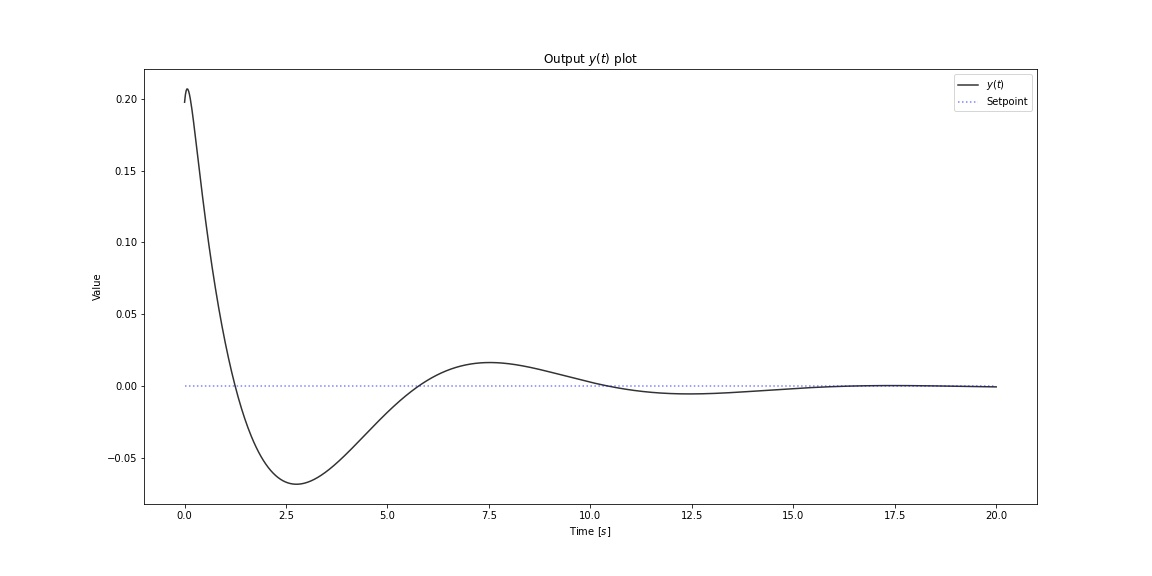
\includegraphics[width=\linewidth]{images/boeing_output.jpg}
\end{figure}

\paragraph{Control input plot} We use the following code for plotting the control input:

\begin{minted}{python}
fig, ax = plt.subplots(1,1, figsize=(16, 8))
ax.plot(t, u, "r", alpha=.8,label=r'$u(t)$')
ax.plot([0, tot_time], [0, 0], ":b", alpha=.5, label=r'Setpoint')
ax.legend(loc='upper right')
ax.set_xlabel(r'Time [$s$]')
ax.set_ylabel(r'Value')
ax.set_title(r"Control input $u(t)$ plot")
fig.savefig('images/boeing_input.jpg')
\end{minted}

\begin{figure}[h!]
    \centering
    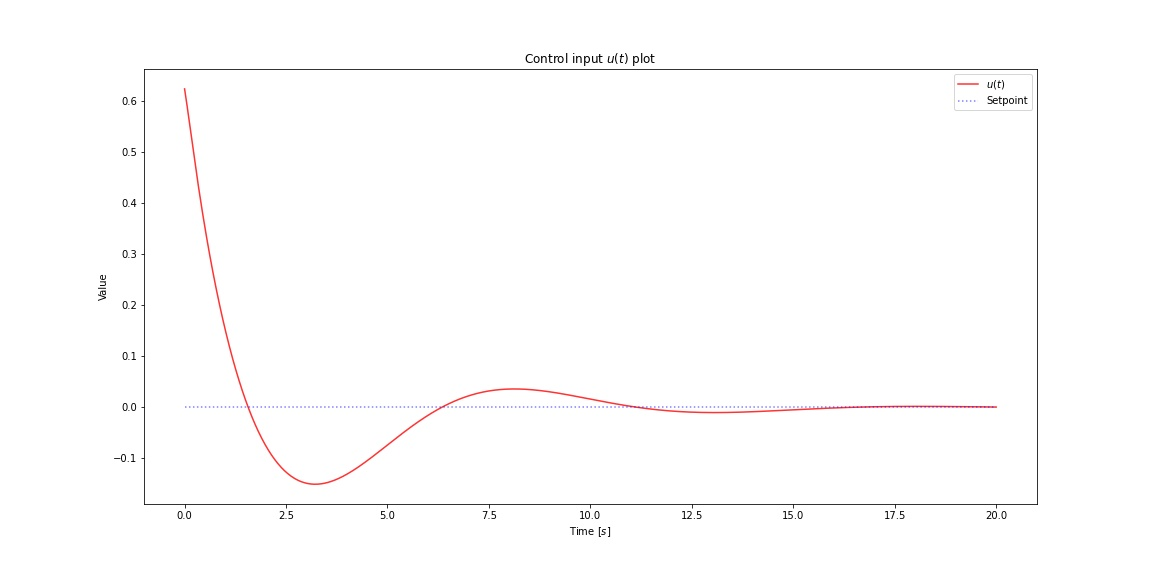
\includegraphics[width=\linewidth]{images/boeing_input.jpg}
\end{figure}

As we can see from the graphs, the LQR controller is able to stabilize the output and bring it to a stable state within the time span we set. Moreover, as we expected, the control input satisfies the condition that $\lim_{t \to \infty} u^*(t) = 0$ and also zeroes out the output in the steady state.